\begin{sidewaysfigure}[ht!]
    \begin{center}
        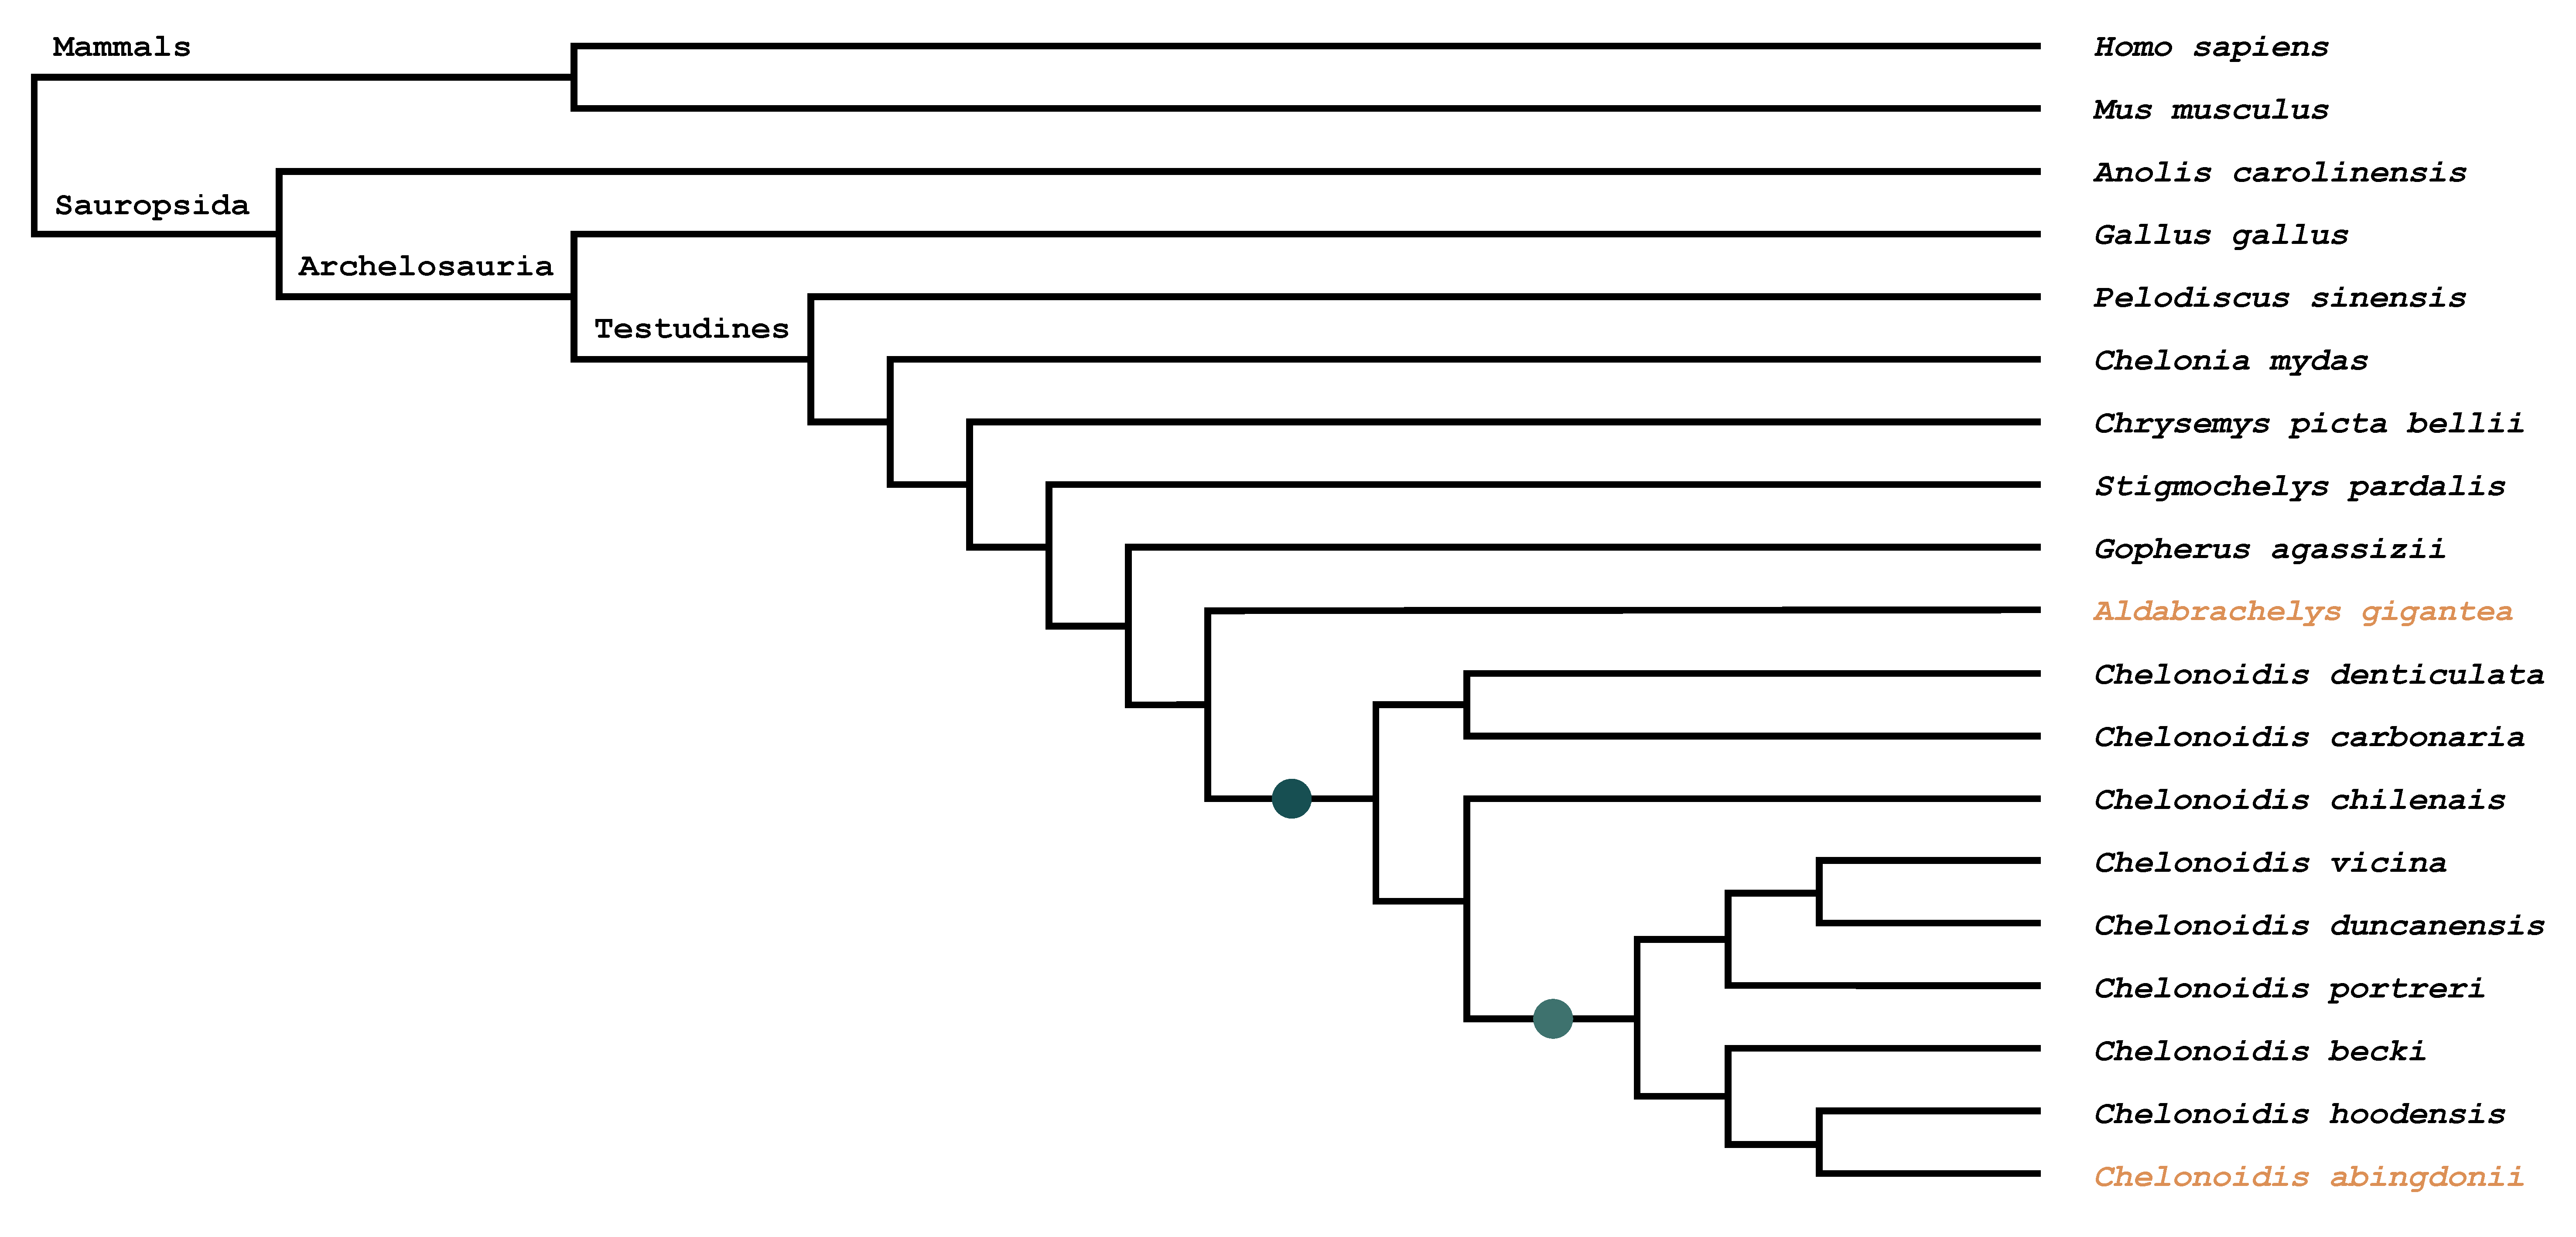
\includegraphics[width=0.9\textwidth]{figures/testudines_tree.pdf}
        \caption[Testudines taxonomy tree]{Testudines taxonomi tree, including the rest of species used in the comparative studies as representatives of the main families comprising the clade of Sauropsida, and \textit{H. sapiens} as the out-group an and reference. Marked in \textcolor{myora1}{\textbf{orange}} are those annotated as part of the present thesis, although punctual annotations for specific genes in the rest were also performed. Closely related tortoises both continental and from the Gal\'{a}pagos archipelago are indicated with the \textcolor{mygre1}{\textbf{darker green}} point, while the radiation of island tortoises is marked using the \textcolor{myaqu1}{\textbf{lighter green}}. Based on the relations shown by \quotes{Time tree} \cite{Kumar2017}.}
        \label{f_testudines_tree}
    \end{center}
\end{sidewaysfigure}
